\documentclass[tikz, border=10pt]{standalone}

%preamble
\usepackage{tikz}

% scale factor
\def\scl{0.6}
% define style
\tikzset{
    % control panel style
    control panel/.style = {draw=black, fill=yellow!30!brown!20!, rounded corners, thick},
    % output screen style
    screen/.style = {draw=black, fill=green!50!black!60!, thick},
    % trace style (graph style)
    trace/.style = {draw=green!60!yellow!40!, ultra thick},
    % small button style
    small button/.style = {draw=black, fill=white, thick},
    % axe style
    axes/.style = {thick}
}

\begin{document}
    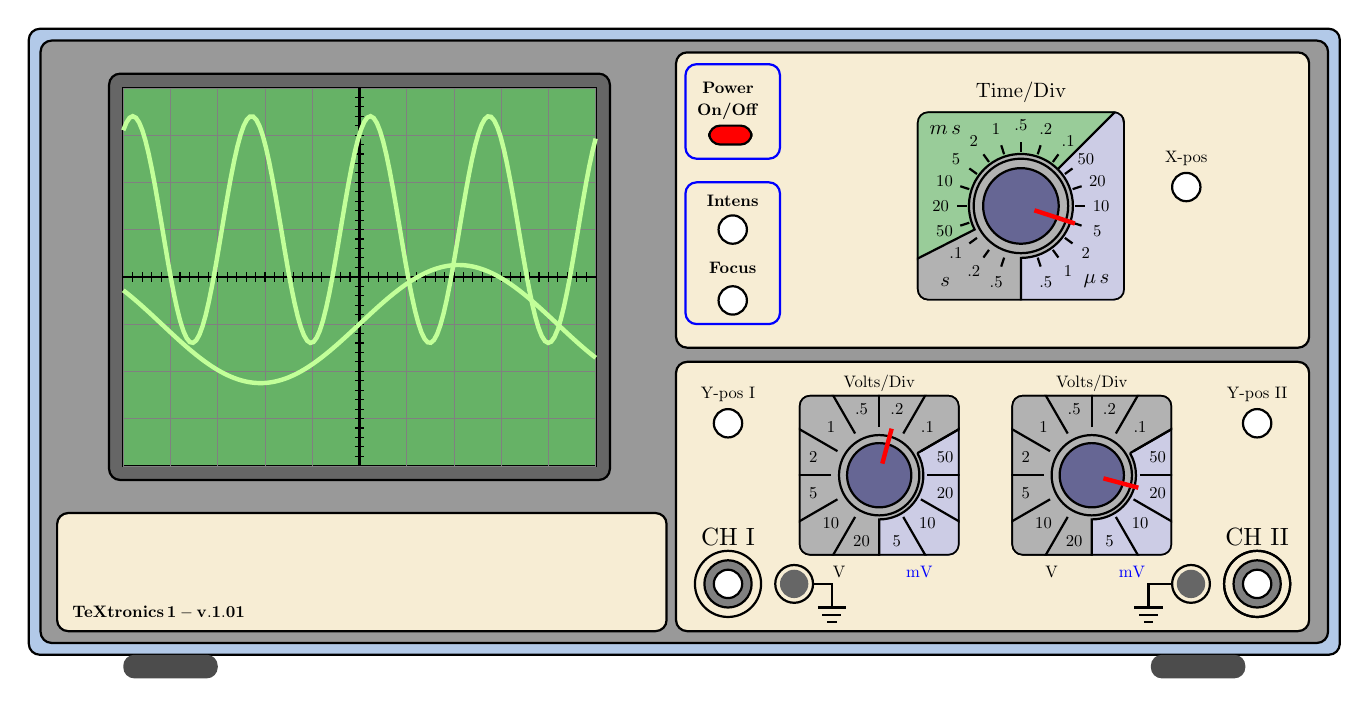
\begin{tikzpicture}[scale=\scl]
        % draw frames and fill the interior of the machine
        \path[draw=black, thick, fill=green!30!blue!30!, rounded corners] (0, 0) rectangle (27.75, 13.25);
        \path[draw=black, thick, fill=black!40!, rounded corners] (0.25, 0.25) rectangle (27.5, 13.00);
        % draw output screen
        % first, shift the coordinate system to (7, 8) - center of the screen
        \begin{scope}[shift={(7cm, 8cm)}, samples=150]
            % draw frames and fill interior of the screen
            \path[fill=black!60!, rounded corners, draw=black, thick](-5.3,-4.3)rectangle (5.3,4.3);
            \path[screen] (-5.0, -4.0) rectangle (5.0, 4.0);
            % draw grid
            \draw[style=help lines] (-5.0, -4.0) grid (5.0, 4.0);
            % draw axe
            \draw[axes] (-5, 0) -- (5, 0);
            \draw[axes] (0, -4) -- (0, 4);
            % draw sticks
            \foreach \i in {-4.8, -4.6, ..., 4.8} \draw (\i, -0.1)--(\i, 0.1);
            \foreach \i in {-3.8, -3.6, ..., 3.8} \draw (-0.1, \i)--(0.1, \i);
            % draw traces (sine lines)
            \draw[trace] plot(\x, {1 + 2.4*sin((2.5*\x + 1) r)});
            \draw[trace] plot(\x, {-1 + 1.25*sin((0.75*\x) r)});
        \end{scope}
        % draw machine stands
        \path[fill=black!70!, draw=none, rounded corners, xshift=2cm] (0, -.5) rectangle (2, 0);
        \path[fill=black!70!, draw=none, rounded corners, xshift=23.75cm] (0, -.5) rectangle (2, 0);
        % draw lower left panel
        \path[control panel] (0.6, 0.5) rectangle (13.5, 3.0);
        \path node [scale=\scl, right] at (0.8, 0.9) {$\mathbf{TeXtronics\,1 - v.1.01}$};
        % draw lower right control panel
        % draw plain panel
        \path[control panel] (13.7, 0.5) rectangle (27.1, 6.2);
        % draw CHI button
        \path[draw, thick] (14.8, 1.5) circle (0.7cm);
        \path[fill=gray, draw=black, thick] (14.8, 1.5) circle (0.5cm);
        \path[fill=white, draw=black, thick] (14.8, 1.5) circle (0.3cm);
        \node[scale={1.5*\scl}] at (14.8, 2.5) {CH I};
        \path[draw, thick] (16.2, 1.5) circle (0.4cm);
        \path[fill=black!60!] (16.2, 1.5) circle (0.3cm);
        \path[draw, thick] (16.6, 1.5) -- (17, 1.5) -- (17, 1.0);
        \path[draw, thick] (16.7, 1.0)--(17.3, 1.0);
        \path[draw, thick] (16.8, 0.85)--(17.2, 0.85);
        \path[draw, thick] (16.9, 0.70)--(17.1, 0.70);
        % draw CHII button
        \path[draw, thick] (26.0, 1.5) circle (0.7cm);
        \path[fill=gray, draw=black, thick] (26, 1.5) circle (0.5cm);
        \path[fill=white, draw=black, thick] (26, 1.5) circle (0.3cm);
        \node[scale={1.5*\scl}] at (26, 2.5) {CH II};
        \path[draw, thick] (24.6, 1.5) circle (0.4cm);
        \path[fill=black!60!] (24.6, 1.5) circle (0.3cm);
        \path[draw, thick] (24.2, 1.5) -- (23.7, 1.5)-- (23.7, 1.0);
        \path[draw, thick] (23.4, 1.0) -- (24.0, 1.0);
        \path[draw, thick] (23.5, 0.85) -- (23.9, 0.85);
        \path[draw, thick] (23.6, 0.70) -- (23.8, 0.70);
        \path[draw, thick] (26.0, 1.5) circle (0.7cm);
        % draw Y-posI small button
        \path[small button] (14.8, 4.9) circle (0.3cm);
        \node[scale=\scl] at (14.8, 5.5) {Y-pos I};
        % draw Y-posII small button
        \path[small button] (26.0, 4.9) circle (0.3cm);
        \node[scale=\scl] at (26.0, 5.5) {Y-pos II};
        % draw left Volt/Div button
        \foreach \pos/\angle in {18/75, 22.5/345}{
            % shift coordinate system to (pos, 3.8) - center of button
            \begin{scope}[xshift=\pos cm, yshift=3.8cm, scale=0.85]
                % add button's name
                \node[scale=\scl] at (0, 2.3) {Volts/Div};
                % draw measures (V and mV)
                \node[scale=\scl, black] at (-1, -2.4) {V};
                \node[scale=\scl, blue]  at (1, -2.4) {mV};
                % clipping the area of button
                \clip[rounded corners] (-2, -2) rectangle (2, 2);
                % fill the button
                \path[fill=black!30!, rounded corners, draw=black, thick] (-2, -2) rectangle (2, 2);
                % fill blue-area of the button
                \path[fill=blue!50!black!20!, draw=black, thick] (30:1.1) -- (30:3) -- (3, -3) -- (-90:3) -- (-90:1.1) arc (-90:30:1.1);
                % draw button
                \path[draw, very thick, rounded corners] (-2, -2) rectangle (2, 2);
                % draw circle button
                \path[draw, thick] (0, 0) circle (1.0 cm);
                % draw sticks
                \foreach \i in {0, 30 , ..., 330}
                    \draw[thick] (\i:1.2)--(\i:2.5);
                % add numbers to the button
                \foreach \i/\j in {15/50, 45/.1, 75/.2, 105/.5, 135/1, 165/2, 195/5, 225/10, 255/20, 285/5, 315/10, 345/20}
                    \node[scale=\scl, black] at (\i:1.7) {\j};
                % fill circle button
                \path[fill=blue!30!black!60!, draw=black, thick] (0,0) circle (0.8cm);
                % draw needle
                \draw[ultra thick, red] (\angle:0.3)--(\angle:1.2);
            \end{scope}
        }
        % draw upper right control panel
        \path[control panel] (13.7, 6.5) rectangle (27.1, 12.75);
        % draw power/off button's frames
        \path[draw, rounded corners, thick, blue] (13.9, 10.5) rectangle (15.9, 12.5);
        % draw power/off button
        \path[fill=red, draw=black, thick, rounded corners] (14.4, 10.8) rectangle (15.3, 11.2);
        % add button name
        \node[scale=\scl] at (14.8, 12) {\textbf{Power}};
        \node[scale=\scl] at (14.8, 11.5) {\textbf{On/Off}};
        % draw Intens and Focus button
        \path[draw, rounded corners, thick, blue] (13.9, 7.0) rectangle (15.9, 10.0);
        \path[small button] (14.9, 7.5) circle (0.3cm);
        \node[scale=\scl] at (14.9, 8.2) {\textbf{Focus}};
        \path[small button] (14.9, 9) circle (0.3cm);
        \node[scale=\scl] at (14.9,9.6) {\textbf{Intens}};
        % draw X-pos button
        \path[small button] (24.5, 9.9) circle (0.3cm);
        \node[scale={\scl}] at (24.5, 10.5) {X-pos};
        % draw Time/Div button
        \begin{scope}[xshift=21cm, yshift=9.5cm, scale=1]
            \node[scale={1.25*\scl}]  at (0, 2.4) {Time/Div};
            \clip[rounded corners] (-2.2, -2) rectangle (2.2, 2);
            \path[fill=black!30!, rounded corners, draw=black, thick] (-2.2, -2) rectangle (2.2, 2);
            \path[fill=blue!50!black!20!, draw=black, thick] (45:1.1) -- (45:3)-- (3, -3) -- (-90:3) -- (-90:1.1) arc (-90:45:1.1);
            \path[fill=green!50!black!40!, draw=black, thick] (45:1.1)-- (45:3) arc (45:207:3) -- (207:1.1) arc (207:45:1.1);
            \path[draw, very thick, rounded corners](-2.2, -2) rectangle (2.2, 2);
            \node[scale={1.25*\scl}] at (-1.6, -1.6) {$s$};
            \node[scale={1.25*\scl}] at (1.6, -1.6) {$\mu{}\,s$};
            \node[scale={1.25*\scl}] at (-1.6, 1.6) {$m\,s$};
            \path[draw, thick] (0, 0) circle (1.0);
            \foreach \i in {-72, -54, ..., 262} \draw[thick] (\i:1.15) -- (\i:1.35);
            \foreach \i/\j in {-72/.5, -54/1 ,-36/2, -18/5, 0/10, 18/20, 36/50, 54/.1, 72/.2, 90/.5,
                    108/1, 126/2, 144/5, 162/10, 180/20, 198/50, 216/.1, 234/.2, 252/.5}
                \node[scale=\scl, black] at (\i:1.7){\j};
            \path[fill=blue!30!black!60!, draw=black, thick] (0, 0) circle (0.8cm);
            \path[draw, ultra thick, red] (-18:0.3) -- (-18:1.2);	
        \end{scope}
    \end{tikzpicture}
\end{document}